\documentclass[11pt]{article}

% Packages
\usepackage[utf8]{inputenc}   % For UTF-8 encoding
\usepackage{amsmath, amssymb} % For mathematical symbols
\usepackage{graphicx}         % For including graphics
\usepackage{geometry}         % For adjusting page dimensions
\usepackage{hyperref}         % For hyperlinks
\usepackage{booktabs}         % For nicer tables
\usepackage{float}            % For figure placement

% Page layout
\geometry{a4paper, margin=1in}

% Document Info
\title{Final Project Report}
\author{Yijia Zhou}
\date{\today}

% Begin Document
\begin{document}

\maketitle


\section{Introduction}
Open Source Energy Modeling System (OSeMOSYS) is an open-source energy modeling system that provides a framework for simulating and optimizing energy systems. It is designed to be flexible and extensible, allowing users to model a wide range of energy technologies and systems. The main goal of OSeMOSYS is to support decision-making in energy planning and policy by providing insights into the costs, emissions, and other impacts of different energy scenarios. Based on the design and development of the OSeMOSYS model \cite{Howells2011}, this project aims to enhance and improve the original open source model by incorporating additional features and functionalities. The project will involve a comprehensive review of the existing model, identification of areas for improvement, and implementation of new features to enhance its capabilities. The final deliverable will be an updated version of the OSeMOSYS model that is more robust, user-friendly, and capable of addressing a wider range of energy modeling scenarios.

\section{Problem Statement}
The problem this model is trying to solve is to optimize the energy system of a given region by minimizing the total cost of energy production and consumption while satisfying a set of constraints related to energy demand, resource availability, and technology characteristics. The model aims to provide insights into the optimal mix of energy technologies and resources that can meet the energy demand of the region while minimizing costs and emissions. 

\section{Background}
\subsection{Objectives}
The main objective is to minimize the total Net Present Value (NPV) of the energy system over the entire planning horizon, which includes both investment costs and operational costs. The model aims to achieve this objective while satisfying a set of constraints related to energy demand, resource availability, and technology characteristics.

\subsection{Assumptions}
We make the assumptions that the energy system is represented as a network of interconnected technologies, each with its own set of characteristics and constraints. The model assumes the parameters and variables are predefined based on the assumptions listed in the next section.

\subsection{Variables and Parameters}
\subsection{Equations}
The model consists of a set of equations that define the relationships between the variables and parameters. The main equations include:
\begin{align}
&\forall_{y,t,r} \; StorageCharge_{s,y,l,r} = 
\sum_{t,m} RateOfActivity_{y,l,t,m,r} 
\times TechnologyToStorage_{t,m,s,r} \times YearSplit_{y,l} \\[1em]
%
&\forall_{y,t,r} \; StorageDischarge_{s,y,l,r} = 
\sum_{t,m} RateOfActivity_{y,l,t,m,r} 
\times TechnologyToStorage_{t,m,s,r} \times YearSplit_{y,l} \\[1em]
%
&\forall_{s,y,l,r} \; NetStorageCharge_{s,y,l,r} = 
StorageCharge_{s,y,l,r} - StorageDischarge_{s,y,l,r} \\[1em]
%
&\forall_{b,s,r} \; StorageLevel_{b,s,r} = 
\sum_{l,y} \left( \frac{NetStorageCharge_{s,y,l,r}}{YearSplit_{y,l}} \right) 
\times StorageInflectionTimes_{y,l,b} \\[1em]
%
&\forall_{b,s,r} \; StorageLowerLimit_{s,r} \leq StorageLevel_{b,s,r} 
\leq StorageUpperLimit_{s,r}
\end{align}

\subsubsection{Inputs}
\begin{itemize}
    \item $Region(r)$: The geographical area being modeled. The example model uses a hypothetical region "UTOPIA".
    \item $Technology(t)$: Each component that can produce, consume, or store energy.
    \begin{itemize}
        \item $E01, E21, E31, E51, E70$: Electricity generation technologies (e.g., coal, gas, nuclear, renewable, diesel).
        \item $IMPDSL1, IMPGSL1, IMPHCO1, IMPOIL1, IMPURN1$: Import technologies for different fuels (e.g., coal, gas, hard coal, oil, uranium).
        \item $RHE, RHO$: Residential heating technologies (electric and diesel-based).
        \item $RL1$: Residential lighting technology.
        \item $TXD, TXE, TXG$: Transmission technologies.
    \end{itemize}
    \item $Year(y)$: Modeled years.
    \item $Timeslice(l)$: Different time periods within a year.
    \begin{itemize}
        \item $Season(ls)$: Different seasons (e.g., winter, summer).
        \item $Daytype(ld)$: Different types of days (e.g., weekday, weekend).
    \end{itemize}
    \item $Fuel(f)$: Types of fuels in this model.
    \begin{itemize}
        \item $DSL$: Diesel
        \item $GSL$: Gasoline
        \item $HCO$: Hard coal
        \item $OIL$: Oil
        \item $HYD$: Hydro
        \item $URN$: Uranium
        \item $RH, RL, TX$: Demand for residential heating, lighting, and transmission.
    \end{itemize}
    \item $Mode(m)$: Different modes of operation for power plants with combined heat and power (CHP) capabilities.
    \item $Daytype(ld)$: Types of days (e.g., weekday, weekend).
    \item $Emissions(e)$: Types of emissions considered in the model (e.g., CO2, NOx).
\end{itemize}

A graphical representation of the Reference Energy System (RES) structure of the OSeMOSYS model is shown in Figure \ref{fig:osemosys_structure} that explains the relationships between fuel imports, electricity generation technologies, residential heating and lighting, and transmission technologies.
\begin{figure}[H]
    \centering
    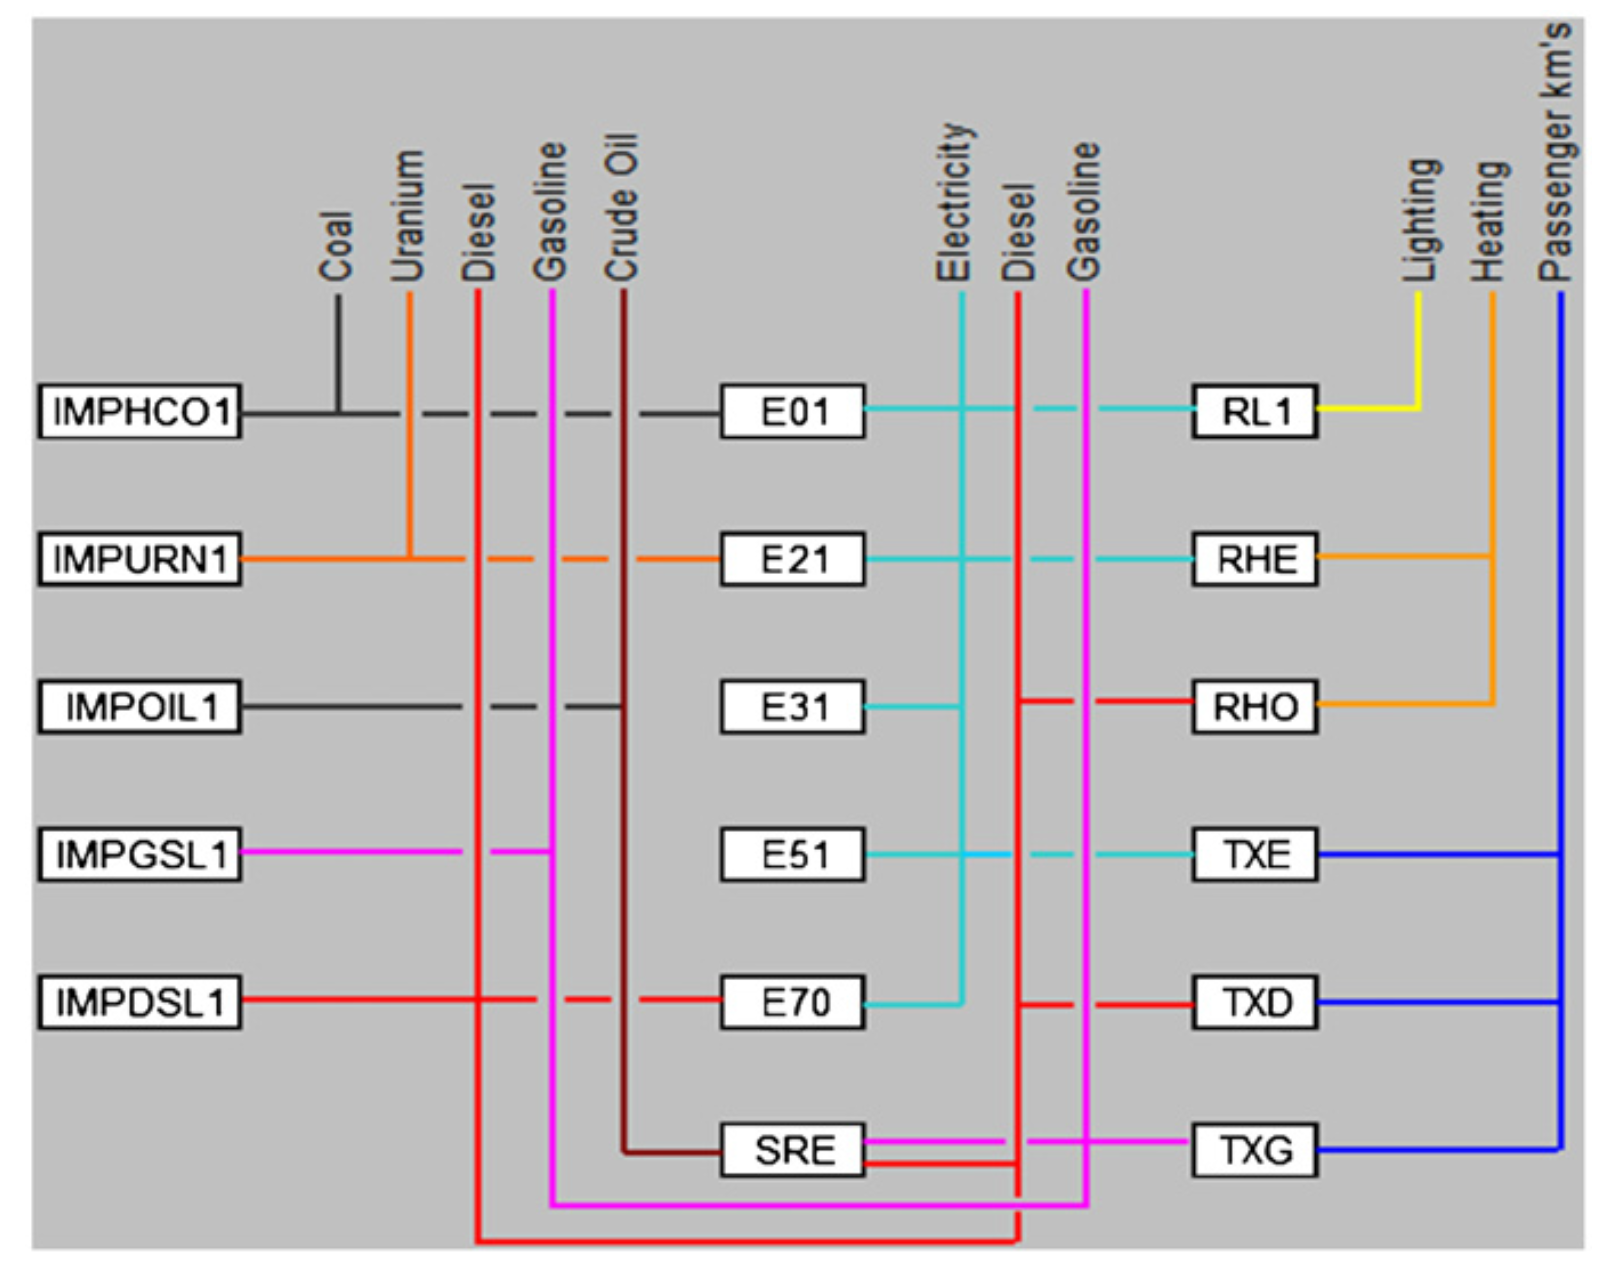
\includegraphics[width=0.8\textwidth]{visualizations/RES}
    \caption{Reference Energy System (RES) structure of the OSeMOSYS model.}
    \label{fig:osemosys_structure}
\end{figure}

\subsection{Parameters}
Below are the parameters that are predefined in the model based on the assumptions.

\subsubsection{Cost}
\begin{itemize}
    \item $VariableCost(y,t,m,r)$: The per-unit cost of operating technology t in year y, mode m, and region r (in \$/PJ).
    \item $FixedCost(y,t,r)$: The fixed cost of technology t in year y and region r (in \$/PJ/year).
    \item $DiscountRate(t,r)$: The discount rate to convert technology t in region r to net value (as a decimal).
    \item $CapitalCost(y,t,r)$: The capital cost of building one unit of technology t in year y and region r (in \$/PJ).
    \item $OperationalLife(t,r)$: The operational life of technology t in region r (in years).
\end{itemize}


\subsection{Storage}
\begin{itemize}
    \item $TechnologyToStorage(t,m,s,r)$: The conversion factor for technology t in mode m and region r to charge per unit.
    \item $TechnologyFromStorage(t,m,s,r)$: The conversion factor for technology t in mode m and region r to discharge per unit.
    \item $YearSplit(y,l)$: The fraction of year y represented by timeslice l (as a decimal).
    \item $StorageInflectionTimes(y,l,b)$: The fraction of year y represented by timeslice l on daytype b (as a decimal).
    \item $StorageLowerLimit(s,r)$: The minimum storage level for storage technology s in region r (in PJ).
    \item $StorageUpperLimit(s,r)$: The maximum storage level for storage technology s in region r (in PJ).
\end{itemize}

\subsection{Capacity}
\begin{itemize}
    \item $ResidualCapacity(t,r)$: The existing capacity of technology t in region r at the start of the model (in PJ year).
    \item $CapacityFactor(y,t,r)$: The capacity factor of technology t in year y and region r (as a decimal).
    \item $CapacityToActivityUnit(t,r)$: The conversion factor from capacity to activity for technology t in region r (in PJ/year).
\end{itemize}


\subsection{Technology Performance}
\begin{itemize}
    \item $OutputActivityRatio(y,t,f,m,r)$: The output activity ratio of technology t in year y, fuel f, mode m, and region r.
    \item $InputActivityRatio(y,t,f,m,r)$: The input activity ratio of technology t in year y, fuel f, mode m, and region r.
\end{itemize}

\subsection{Demand}
\begin{itemize}
    \item $AccumulatedAnnualDemand(y,t,r)$: The accumulated annual demand for technology t in year y and region r (in MWh).
\end{itemize}

\subsection{Capacity and Activity Limits}
\begin{itemize}
    \item $TotalAnnualMaxCapacity(y,t,r)$: The total annual maximum capacity for technology t in year y and region r (in MW).
    \item $TotalAnnualMaxCapacityInvestment(y,t,r)$: The total annual maximum capacity investment for technology t in year y and region r (in MW).
    \item $TotalTechnologyAnnualActivityUpperLimit(y,t,r)$: The total technology annual activity upper limit for technology t in year y and region r (in MWh).
    \item $TotalTechnologyAnnualActivityLowerLimit(y,t,r)$: The total technology annual activity lower limit for technology t in year y and region r (in MWh).
    \item $TotalTechnologyModelPeriodActivityUpperLimit(t,r)$: The total technology model period activity upper limit for technology t in region r (in MWh).
    \item $TotalTechnologyModelPeriodActivityLowerLimit(t,r)$: The total technology model period activity lower limit for technology t in region r (in MWh).
\end{itemize}

\subsection{Reserve Margin}
\begin{itemize}
    \item $ReserveMarginTagTechnology(y,t,r)$: The fraction of reserve margin for technology t in year y and region r to contribute to meet the margin (as a decimal).
    \item $ReserveMarginTagFuel(y,f,r)$: The fraction of reserve margin for fuel f in year y and region r to contribute to meet the margin (as a decimal).
    \item $ReserveMargin(y,r)$: The required fraction of reserve margin for year y and region r (as a decimal).
\end{itemize}

\subsection{Emissions}
\begin{itemize}
    \item $EmissionActivityRatio(y,t,m,e,r)$: The fraction of emissions for technology t in year y, mode m, and region r (as a decimal).
    \item $EmissionPenalty(y,e,r)$: The emission intensity for technology t in year y, mode m, and region r (as a decimal).
    \item $AnnualExogenousEmission(y,e,r)$: The total annual emissions for region r in year y for emission type e (in tCO2, tNOx).
    \item $ModelPeriodExogenousEmission(e,r)$: The total model period emissions for region r for emission type e (in tCO2, tNOx).
    \item $AnnualEmissionLimit(y,e,r)$: The annual emission limit for region r in year y for emission type e (in tCO2, tNOx).
    \item $ModelPeriodEmissionLimit(e,r)$: The model period emission limit for region r for emission type e (in tCO2, tNOx).
\end{itemize}

\subsection{Implementation}
I am using an open-source implementation of OSeMOSYS in github \cite{githubrepo} that is written in Python. The implementation \cite{Dreier2019} uses the PuLP library to define and solve the optimization model.

\subsection{Verification and Testing}
There is not real verification as the real-world scenarios does not necessarily follow the minimized cost this model aims to achieve. However, I want to use the published data from 2010 to 2020 to see how well the model can predict the energy system's behavior during this period. I will compare the model's output with the actual data to assess its accuracy and reliability.


\section{Methods}
\subsection{Model Setup}
I have successfully set up the OSeMOSYS model using the open-source implementation in Python. I have defined the model's parameters, variables, and constraints based on the assumptions and objectives outlined in the background section.

\subsection{Visualization}
The model itself does not have a built-in visualization tool. However, I have created some visualizations using Python libraries such as Matplotlib to help analyze and interpret the model's output. For example, I have created plots showing the Total Capacity by Technology over the years, as shown in Figure \ref{fig:total_capacity}, Total Technology Capacity over time, as shown in Figure \ref{fig:total_technology_capacity}.
\begin{figure}[H]
    \centering
    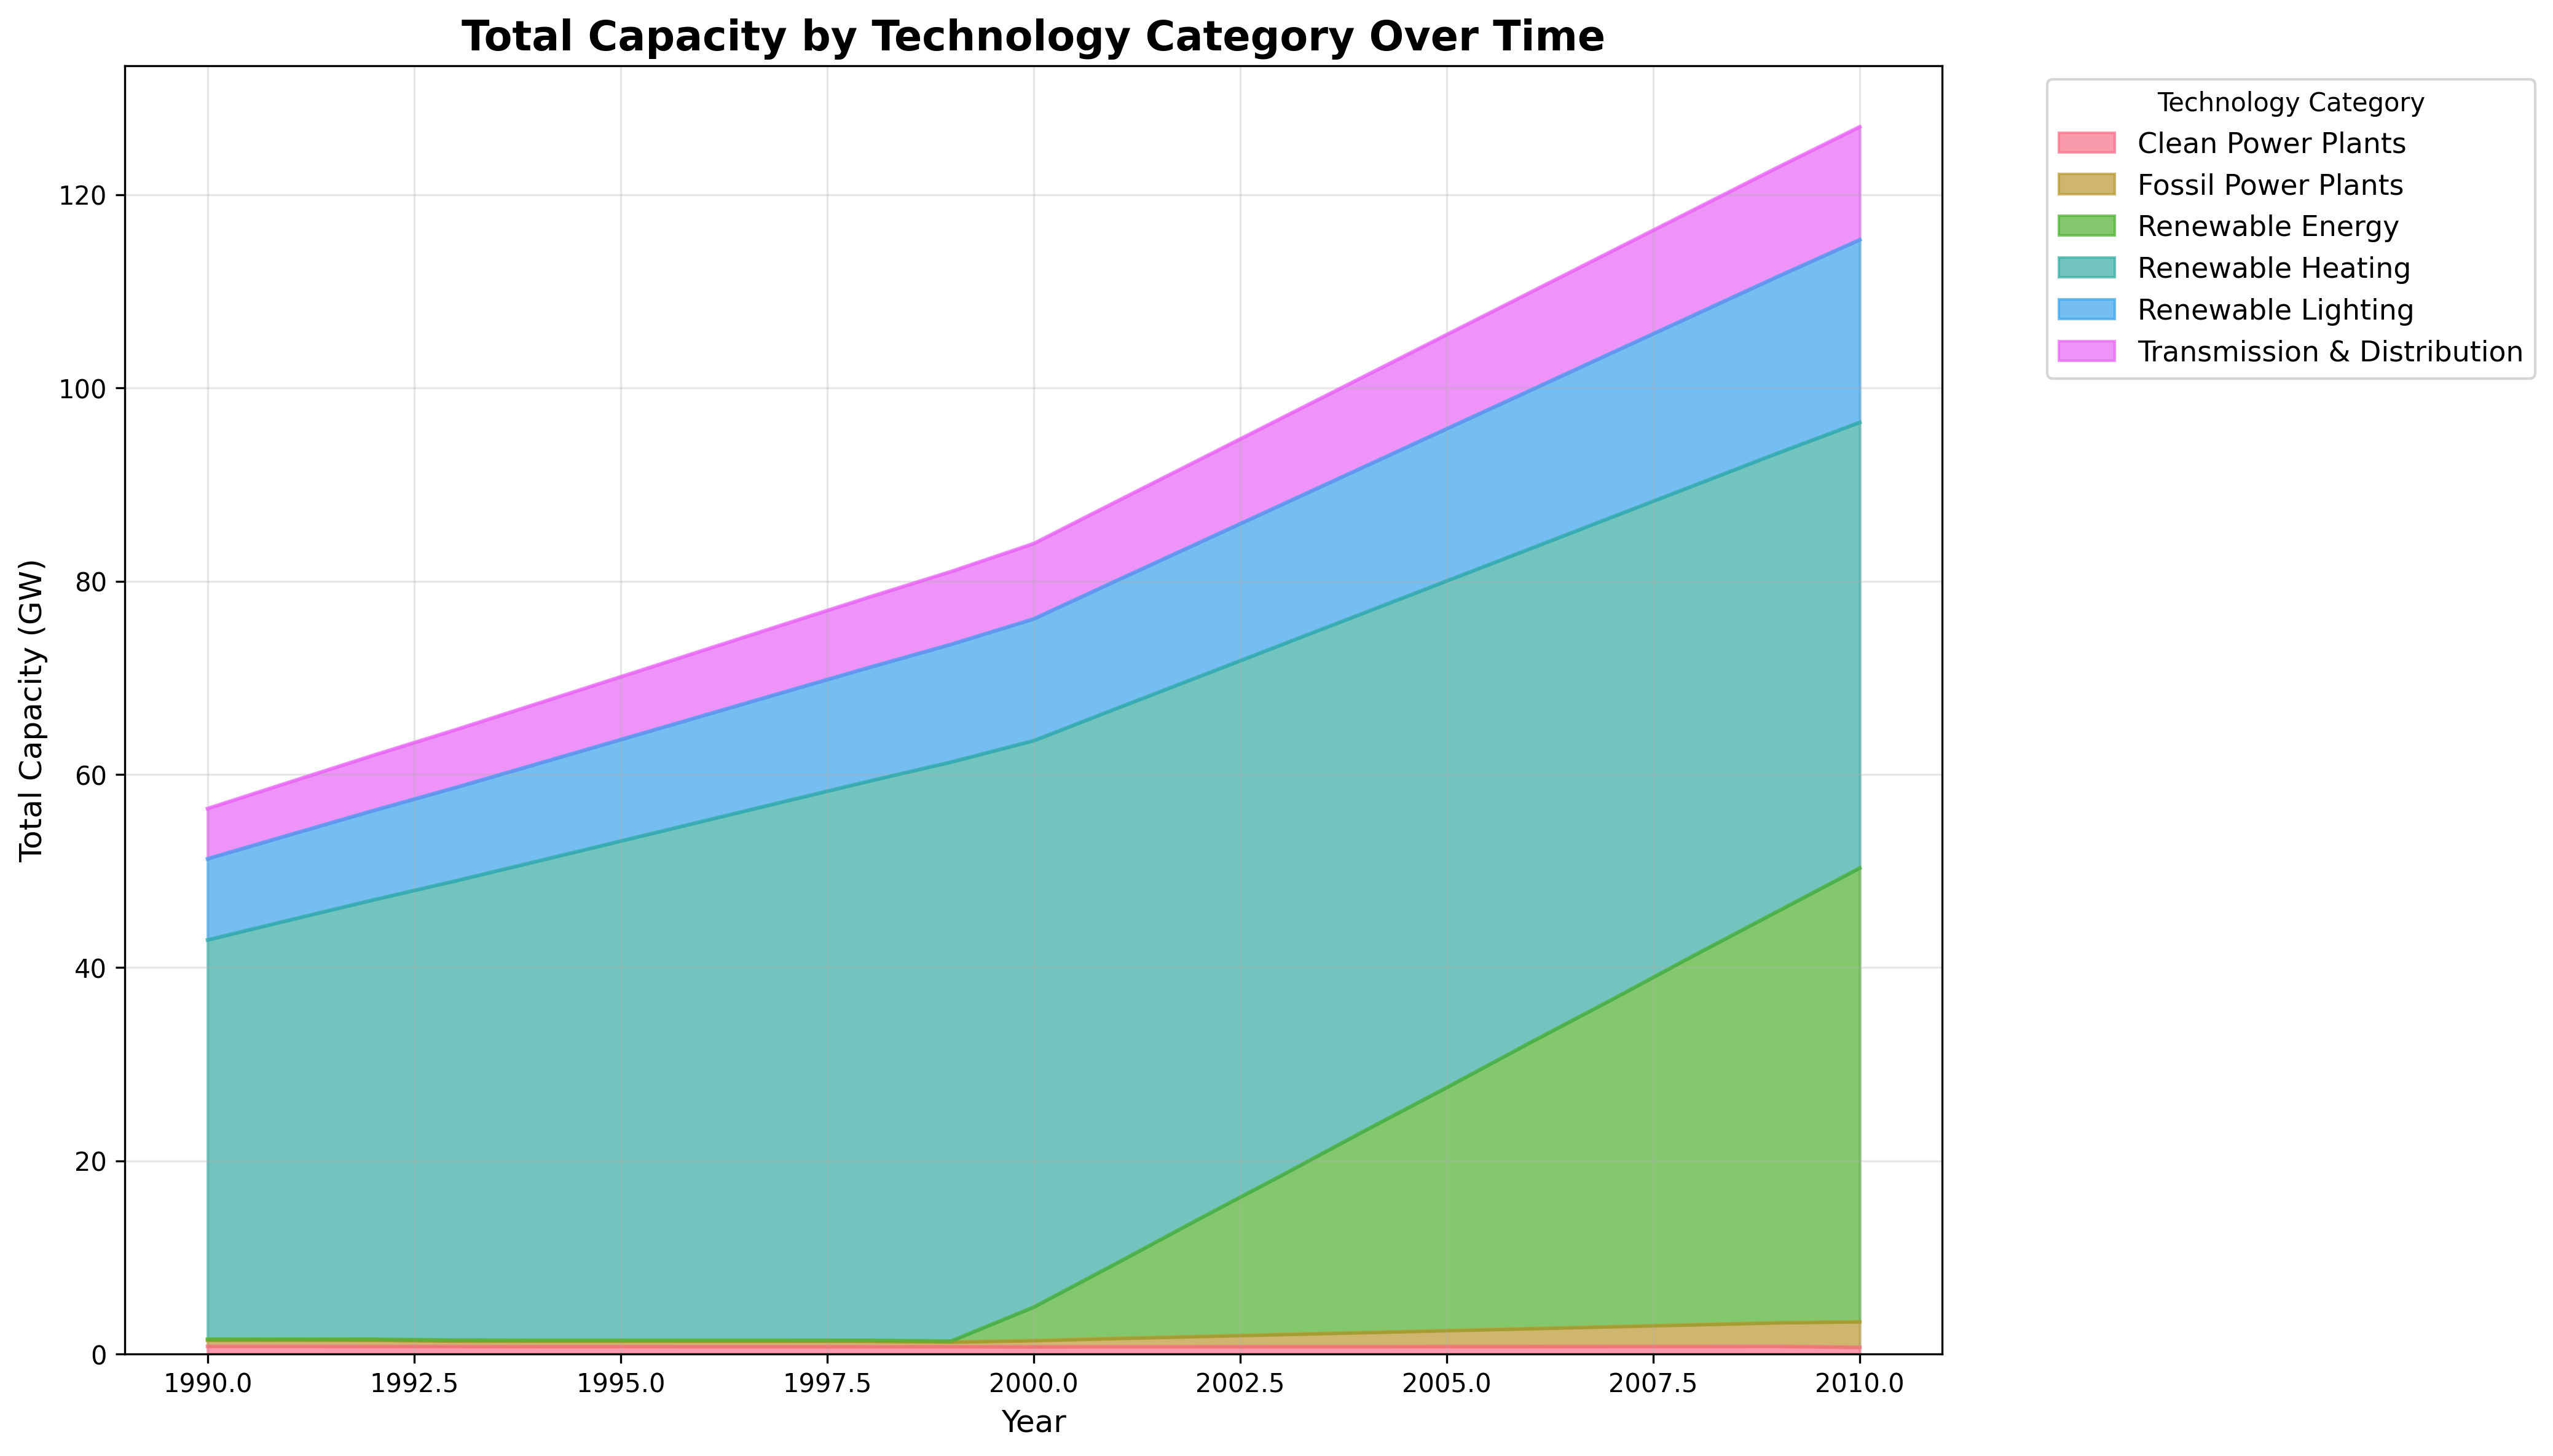
\includegraphics[width=0.8\textwidth]{visualizations/capacity_by_category_labeled.png}
    \caption{Total Capacity by Technology over the years.}
    \label{fig:total_capacity}
\end{figure}

\begin{figure}[H]
    \centering
    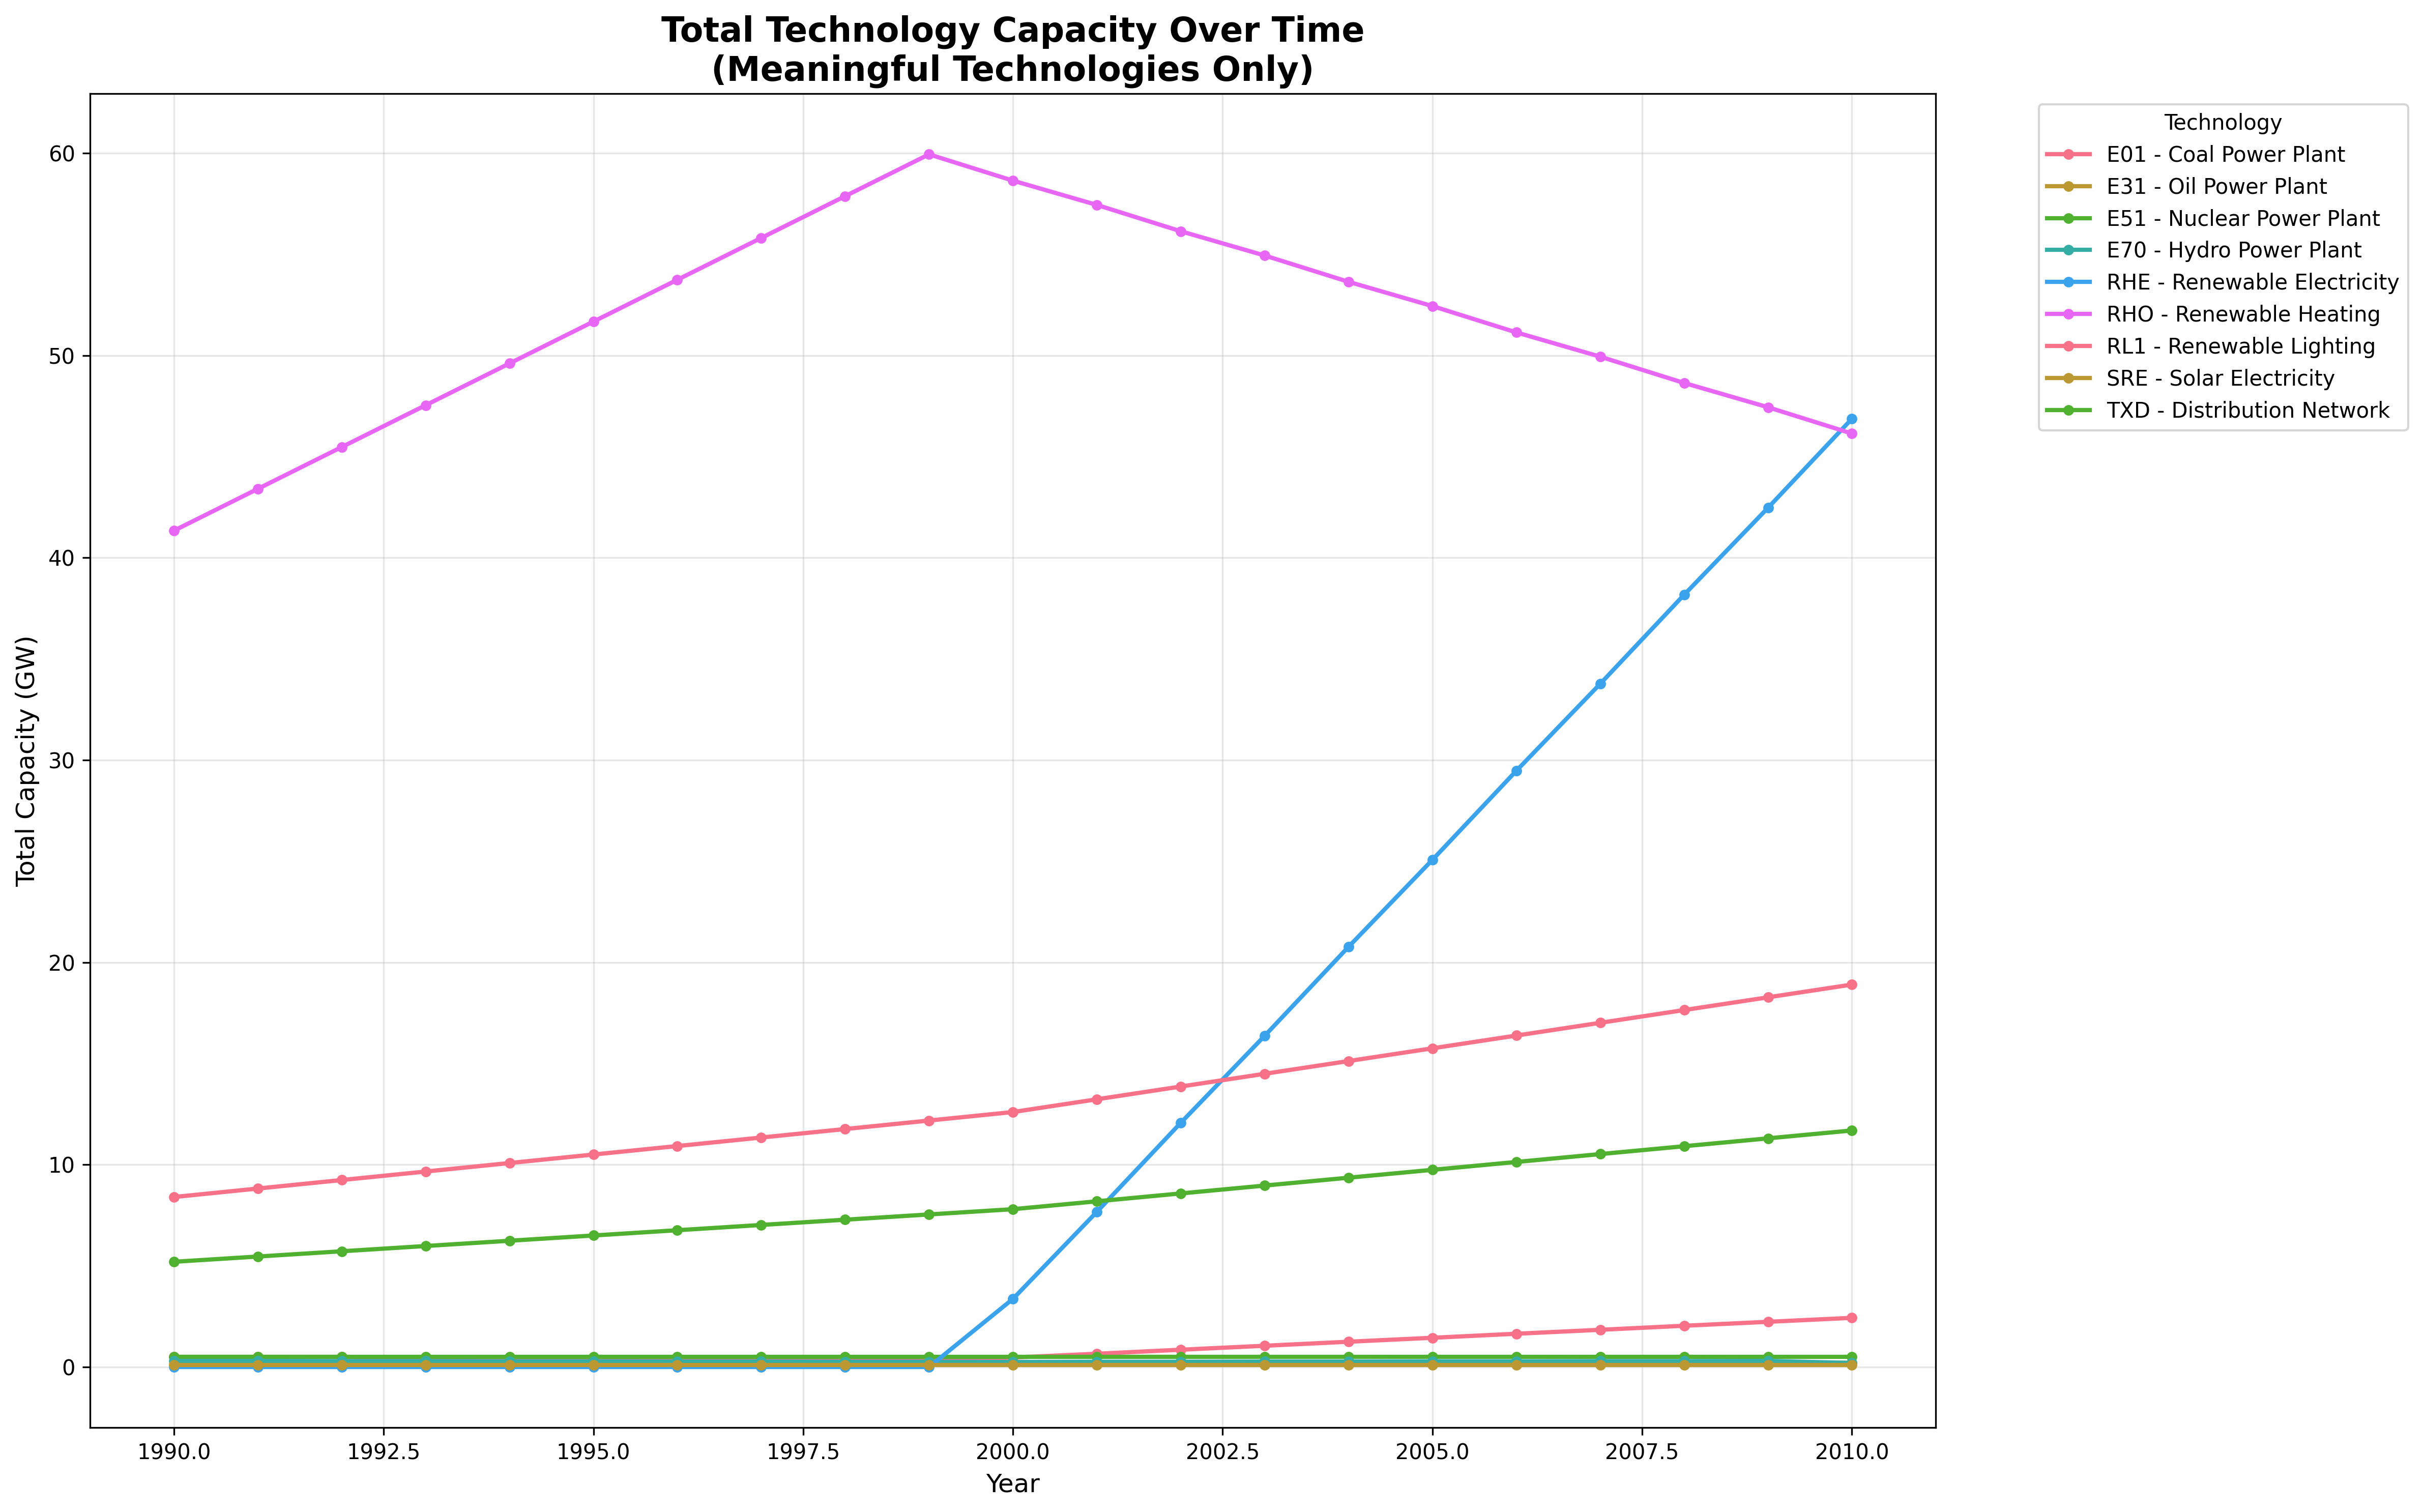
\includegraphics[width=0.8\textwidth]{visualizations/meaningful_total_capacity_labeled.png}
    \caption{Total Technology Capacity over time.}
    \label{fig:total_technology_capacity}
\end{figure}

As for the optimized result, I have created the New Technology Investment over time, as shown in Figure \ref{fig:new_technology_investment} and \ref{fig:capital_investment}.
\begin{figure}[H]
    \centering
    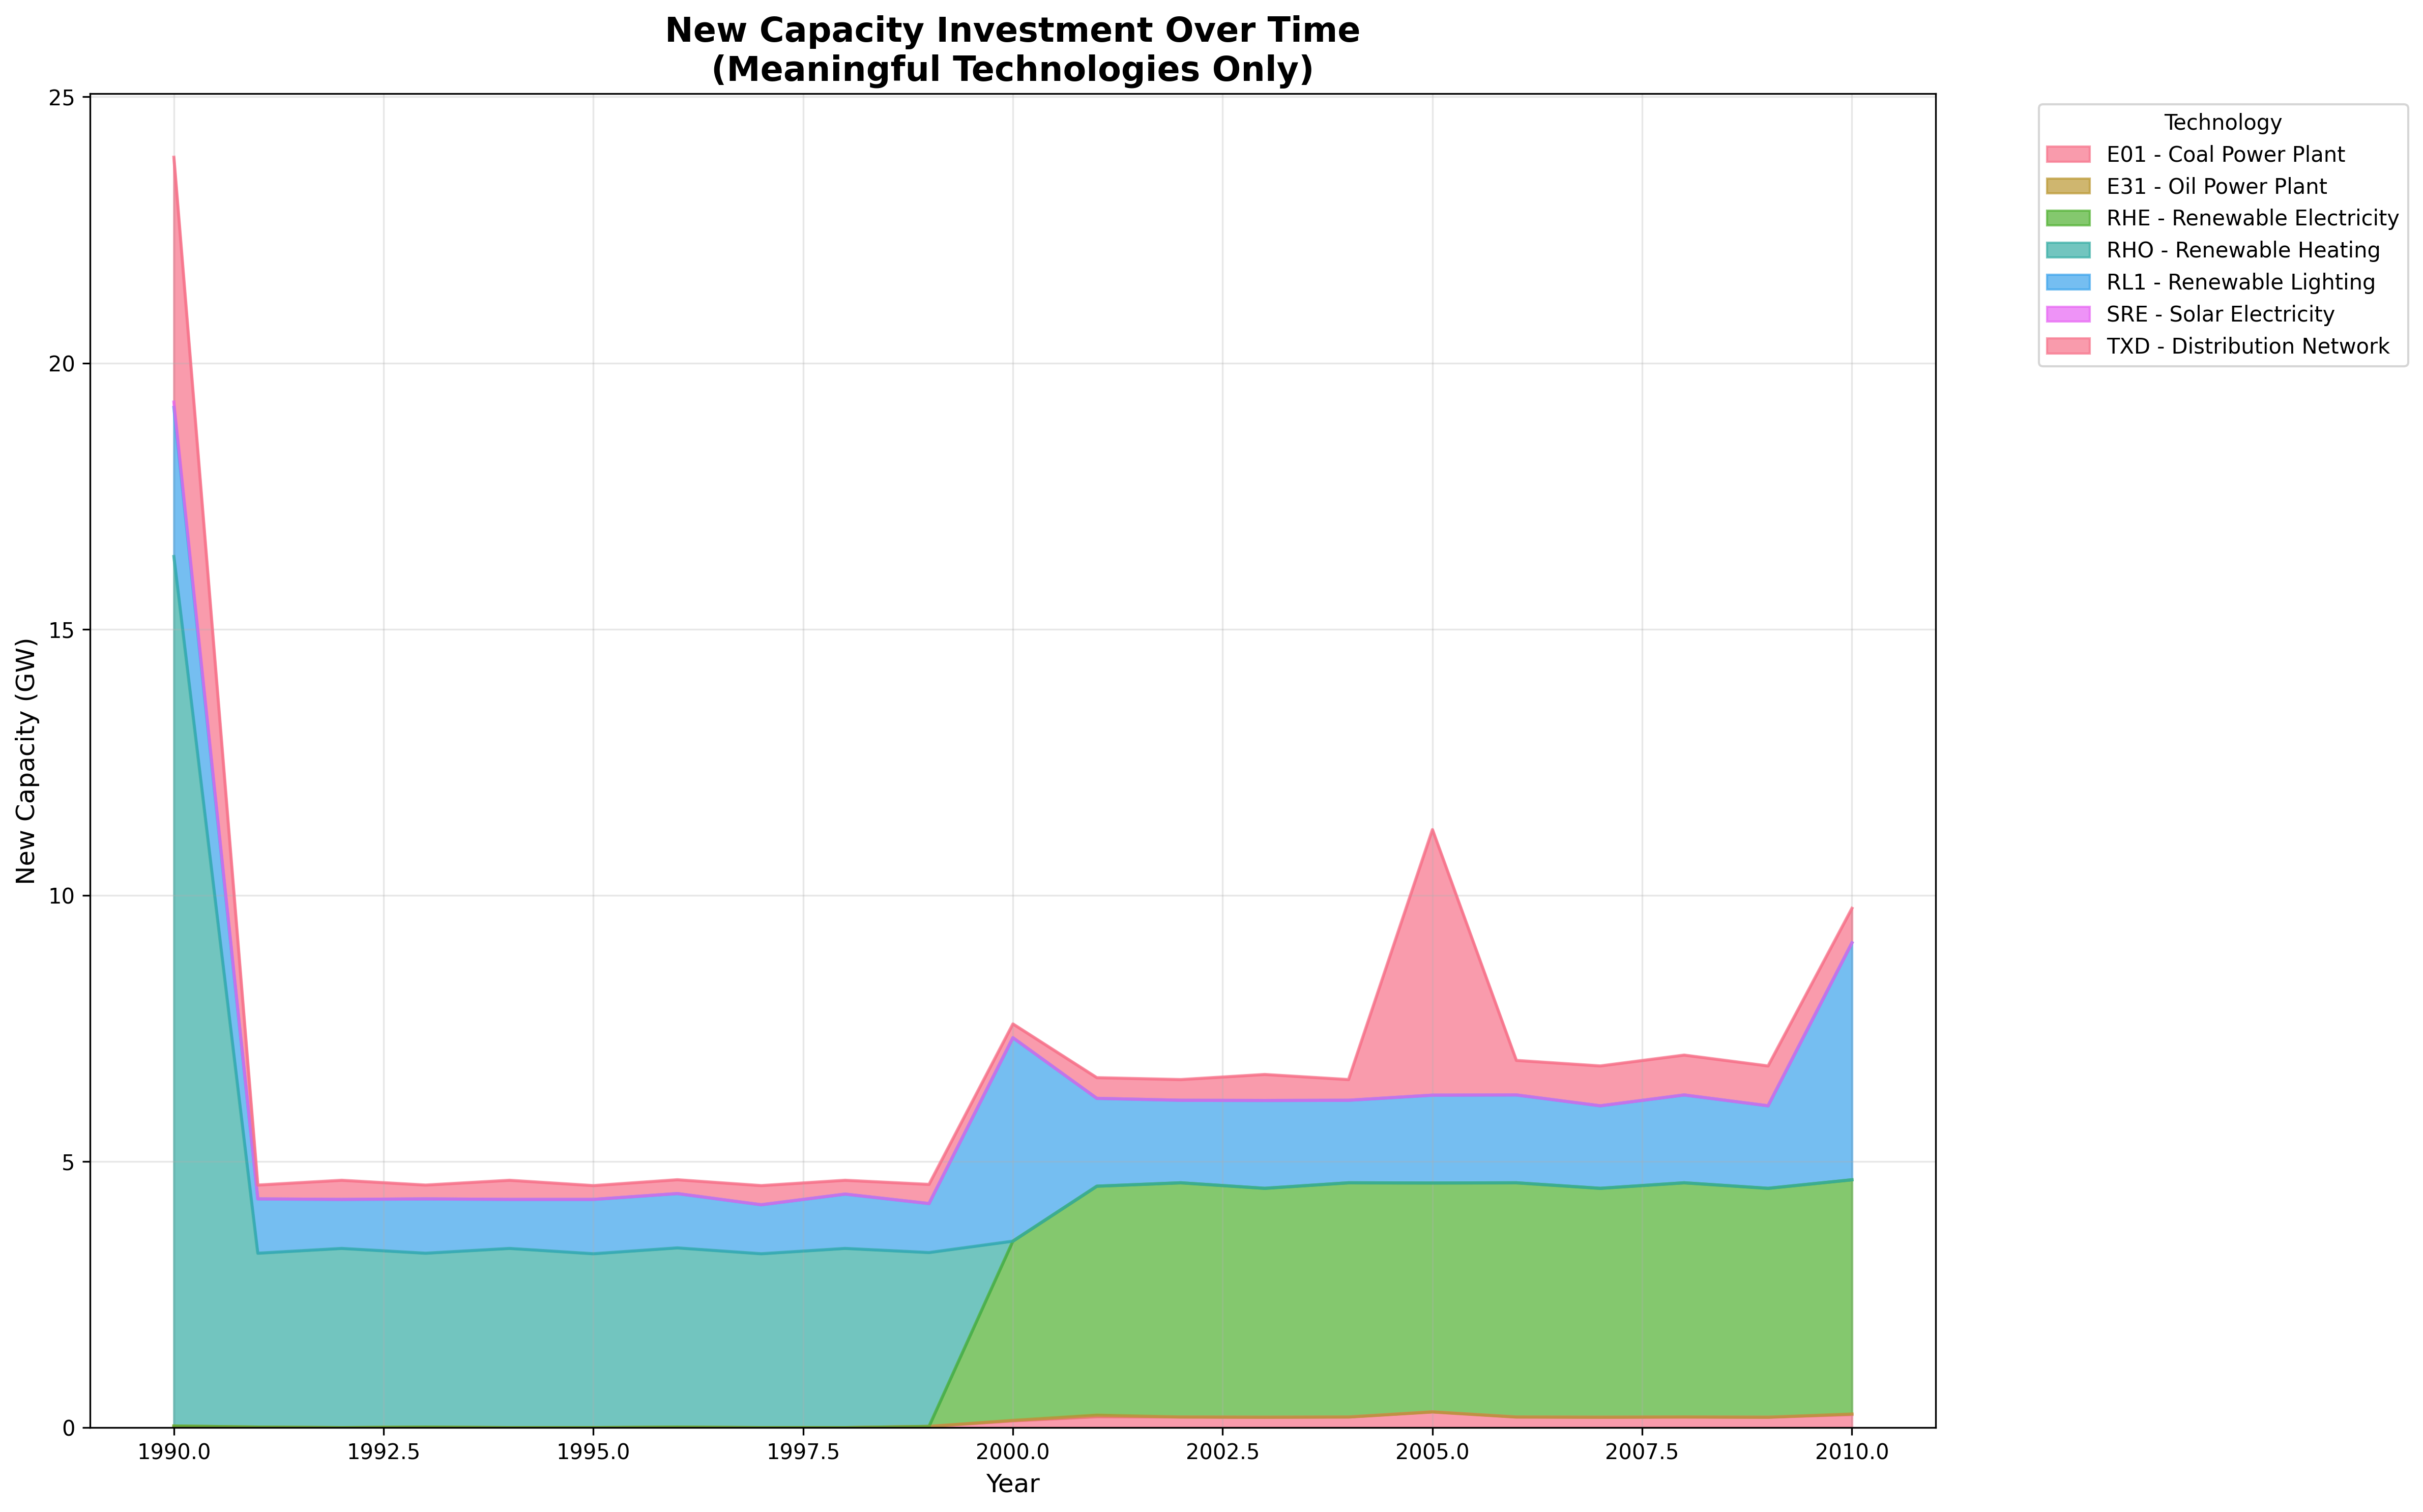
\includegraphics[width=0.8\textwidth]{visualizations/meaningful_technology_capacity_labeled.png}
    \caption{New Technology Investment over time.}
    \label{fig:new_technology_investment}
\end{figure}    

\begin{figure}[H]
    \centering
    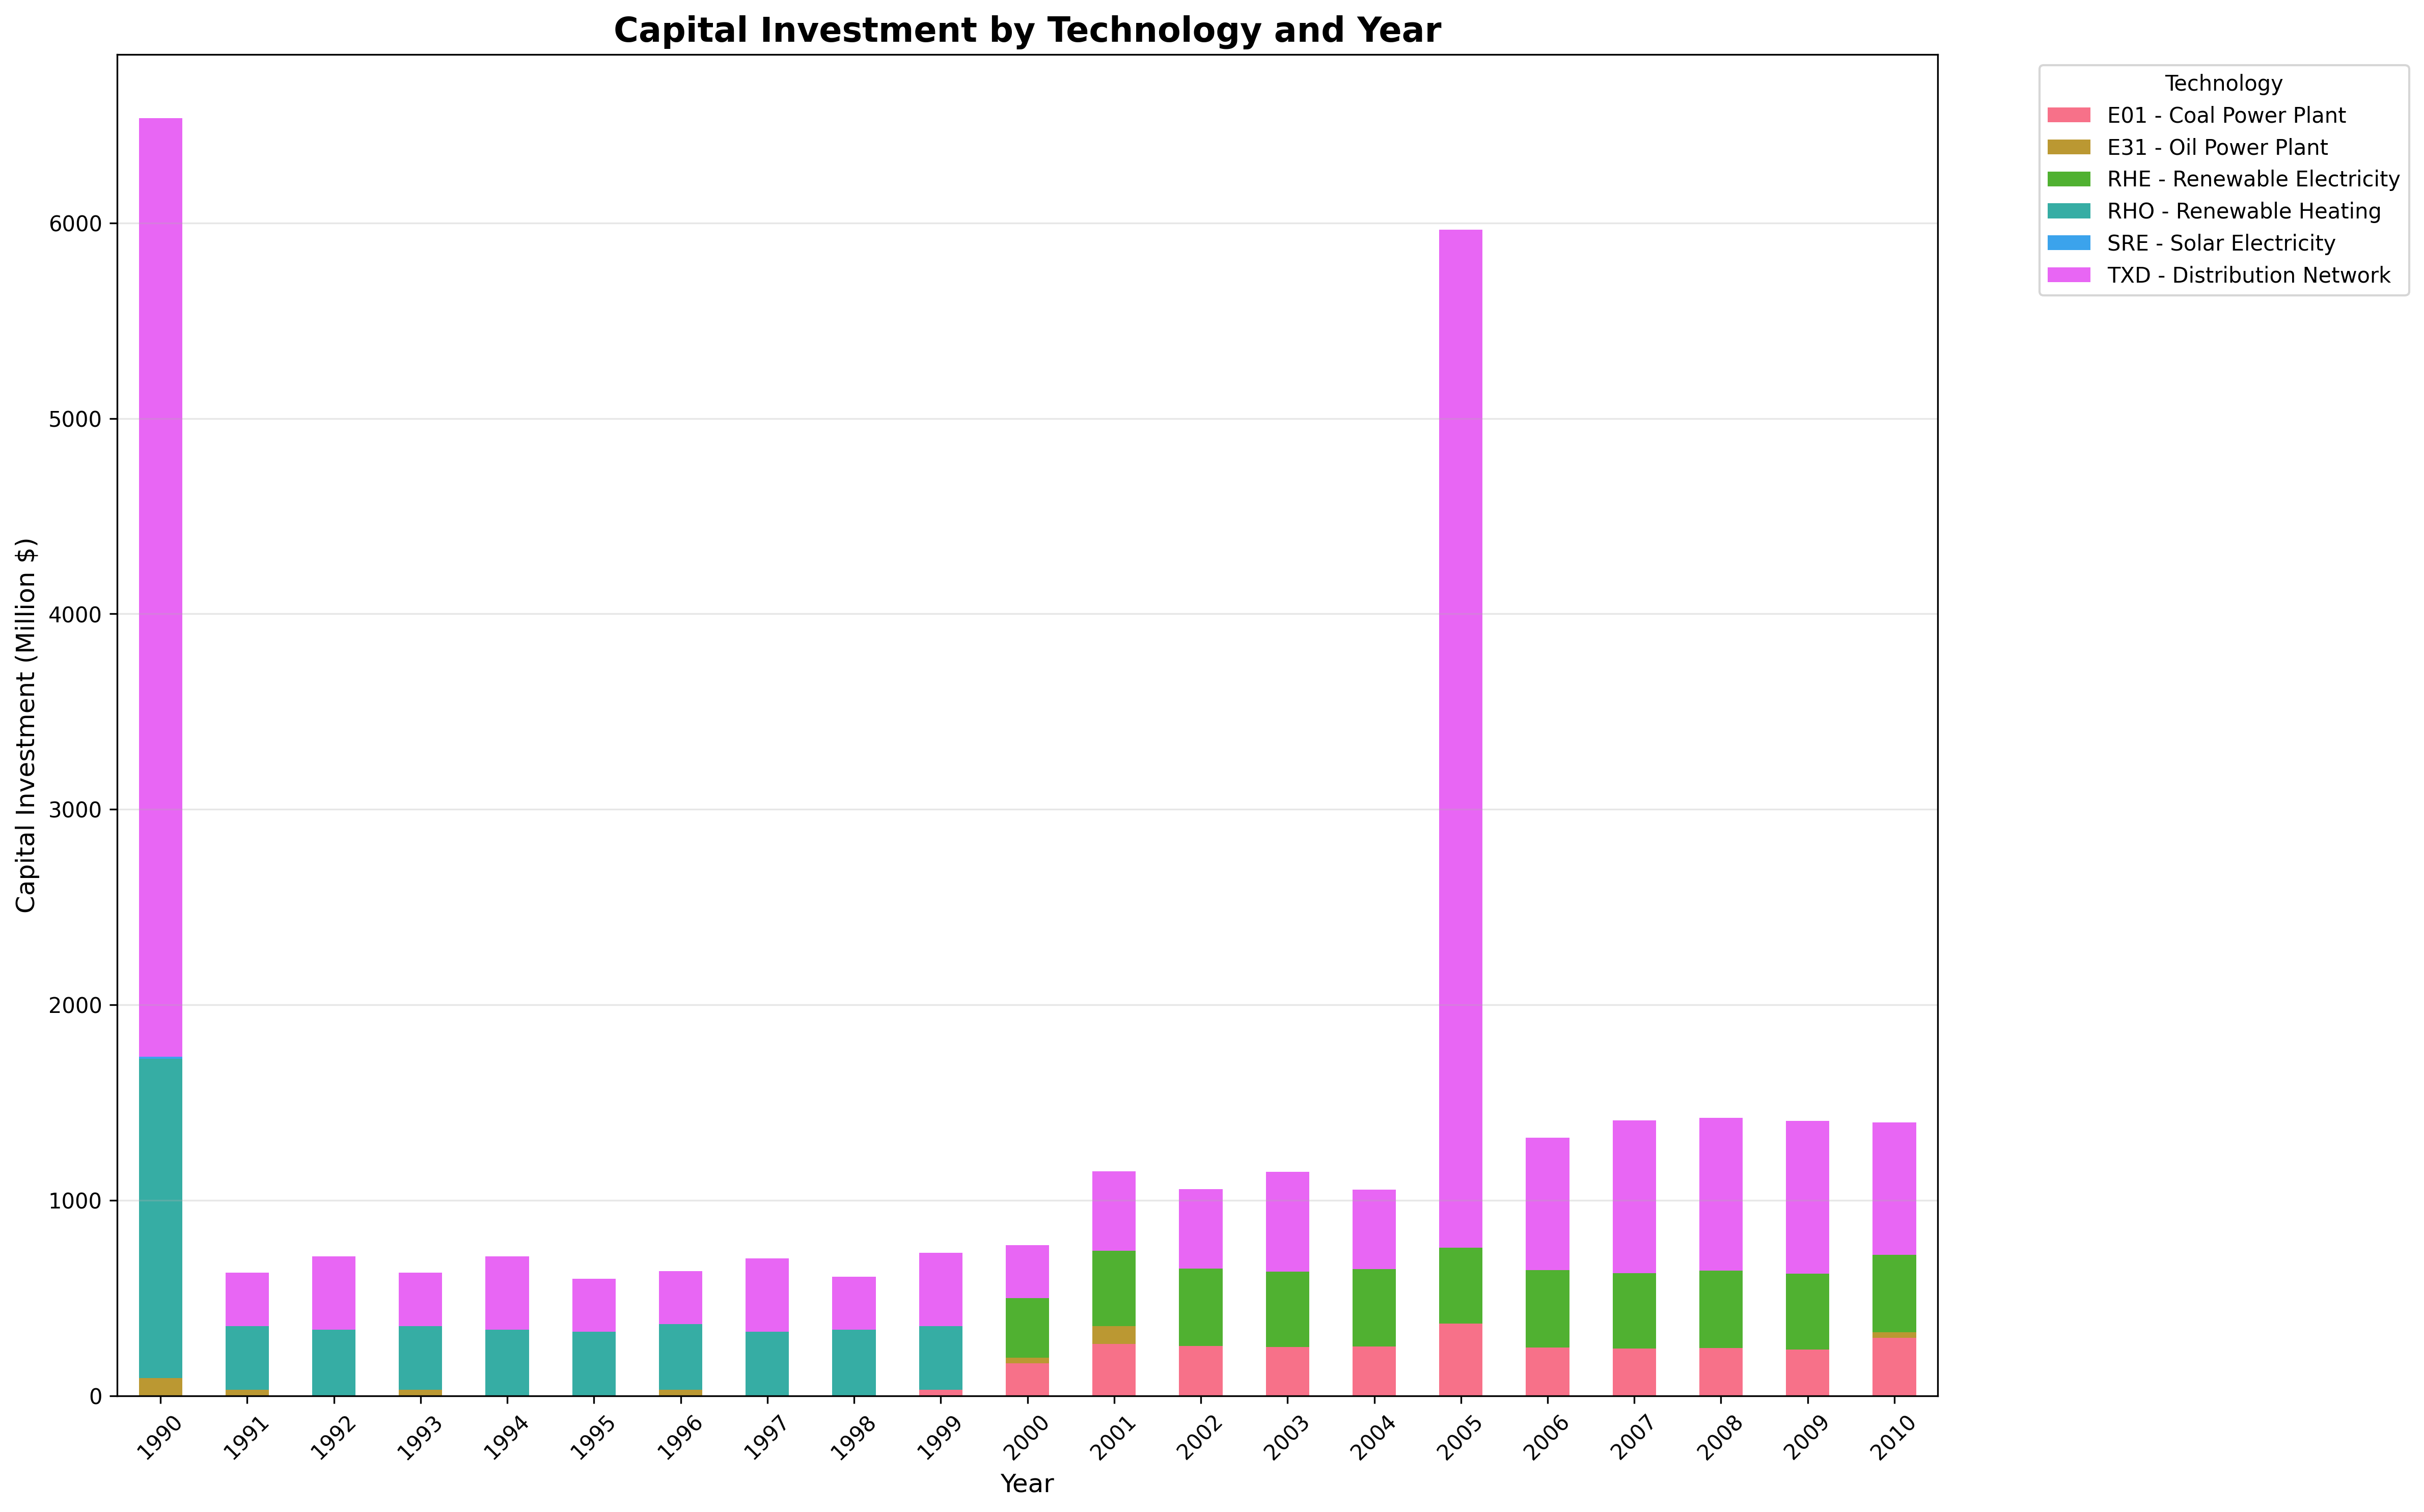
\includegraphics[width=0.8\textwidth]{visualizations/capital_investment_labeled.png}
    \caption{Capital Investment over time.}
    \label{fig:capital_investment}
\end{figure}    

\section{Enhancements}
\subsection{Model Enhancement}
I try to enhance the model by incorporating additional features and functionalities. This change includes adding charge and discharge efficiencies for storage technologies, creating comprehensive testing and visualization functionalities. 

\subsection{Comparison with Real-World Data}
At the same time, I also collected real-world data to compare the model's predictions with actual outcomes. However, due to the legacy data lacking details on certain technologies, I only used the latest data from 2022 to 2023 in the US to compare with the model's output. The data needs to be transformed as there is not an exact one to one mapping relationships for a lot of variables like the technologies used in the real world mapping to the model. The comparison results are shown in Figure \ref{fig:real_world_comparison}. We notice that the model does not cover all technologies in the real world, expecially the renewable sources excluding hydroelectricity like Solar Thermal and Photovoltaic. However, the model does capture the general trend of the energy system, such as the dominance of natural gas and coal in electricity generation. And for that part the energy imports and consumptions are quite close to the real-world data.
There are two major missing technologies in the model compared to the real world.
\begin{itemize}
    \item Natural Gas (38.0\% of US generation) - No gas as the import in current model.
    \item Wind (8.9\% of US generation) - No wind technology in current model.
\end{itemize}

And the data also have some limitations including:
\begin{itemize}
    \item Real world data is from EPA (2022-2023) while model data is from OSeMOSYS (1990-2010)
    \item Model uses UTOPIA reference system, not US electricity grid
    \item Power generation comparison: Model uses ideal E-series power plants for simplification
    \item Different units and scales between datasets require careful interpretation
    \item Real world data represents actual electricity generation in TWh
    \item Model data represents capacity and fuel use in model-specific units
    \item Filtered out unrealistic model values ($\geq$ 1000) which appear to be upper bound constraints
    \item Import technologies (IMP*) had constraint values of 99999, not actual capacities
\end{itemize}



\begin{table}[H]
    \centering
    \begin{tabular}{ll}
        \toprule
        REAL WORLD DATA ANALYSIS (2022-2023) \\
        \midrule
        Total Electricity Generation 2023: 4754.2 TWh \\
        Total Electricity Generation 2022: 4791.9 TWh \\
        Year-over-year change: -0.79\% \\
        \midrule
        Top Electricity Generation Sources (2023): \\
         $\bullet$ Natural Gas: 1806.1 TWh (38.0\%) \\
         $\bullet$ Nuclear: 774.9 TWh (16.3\%) \\
         $\bullet$ Coal: 675.1 TWh (14.2\%) \\
         $\bullet$ Renewables\_Excl\_Hydro: 650.2 TWh (13.7\%) \\
         $\bullet$ Wind: 421.1 TWh (8.9\%) \\
        \bottomrule
    \end{tabular}
    \caption{REAL WORLD vs OSeMOSYS MODEL COMPARISON REPORT}
\end{table}

\begin{figure}[H]
    \centering
    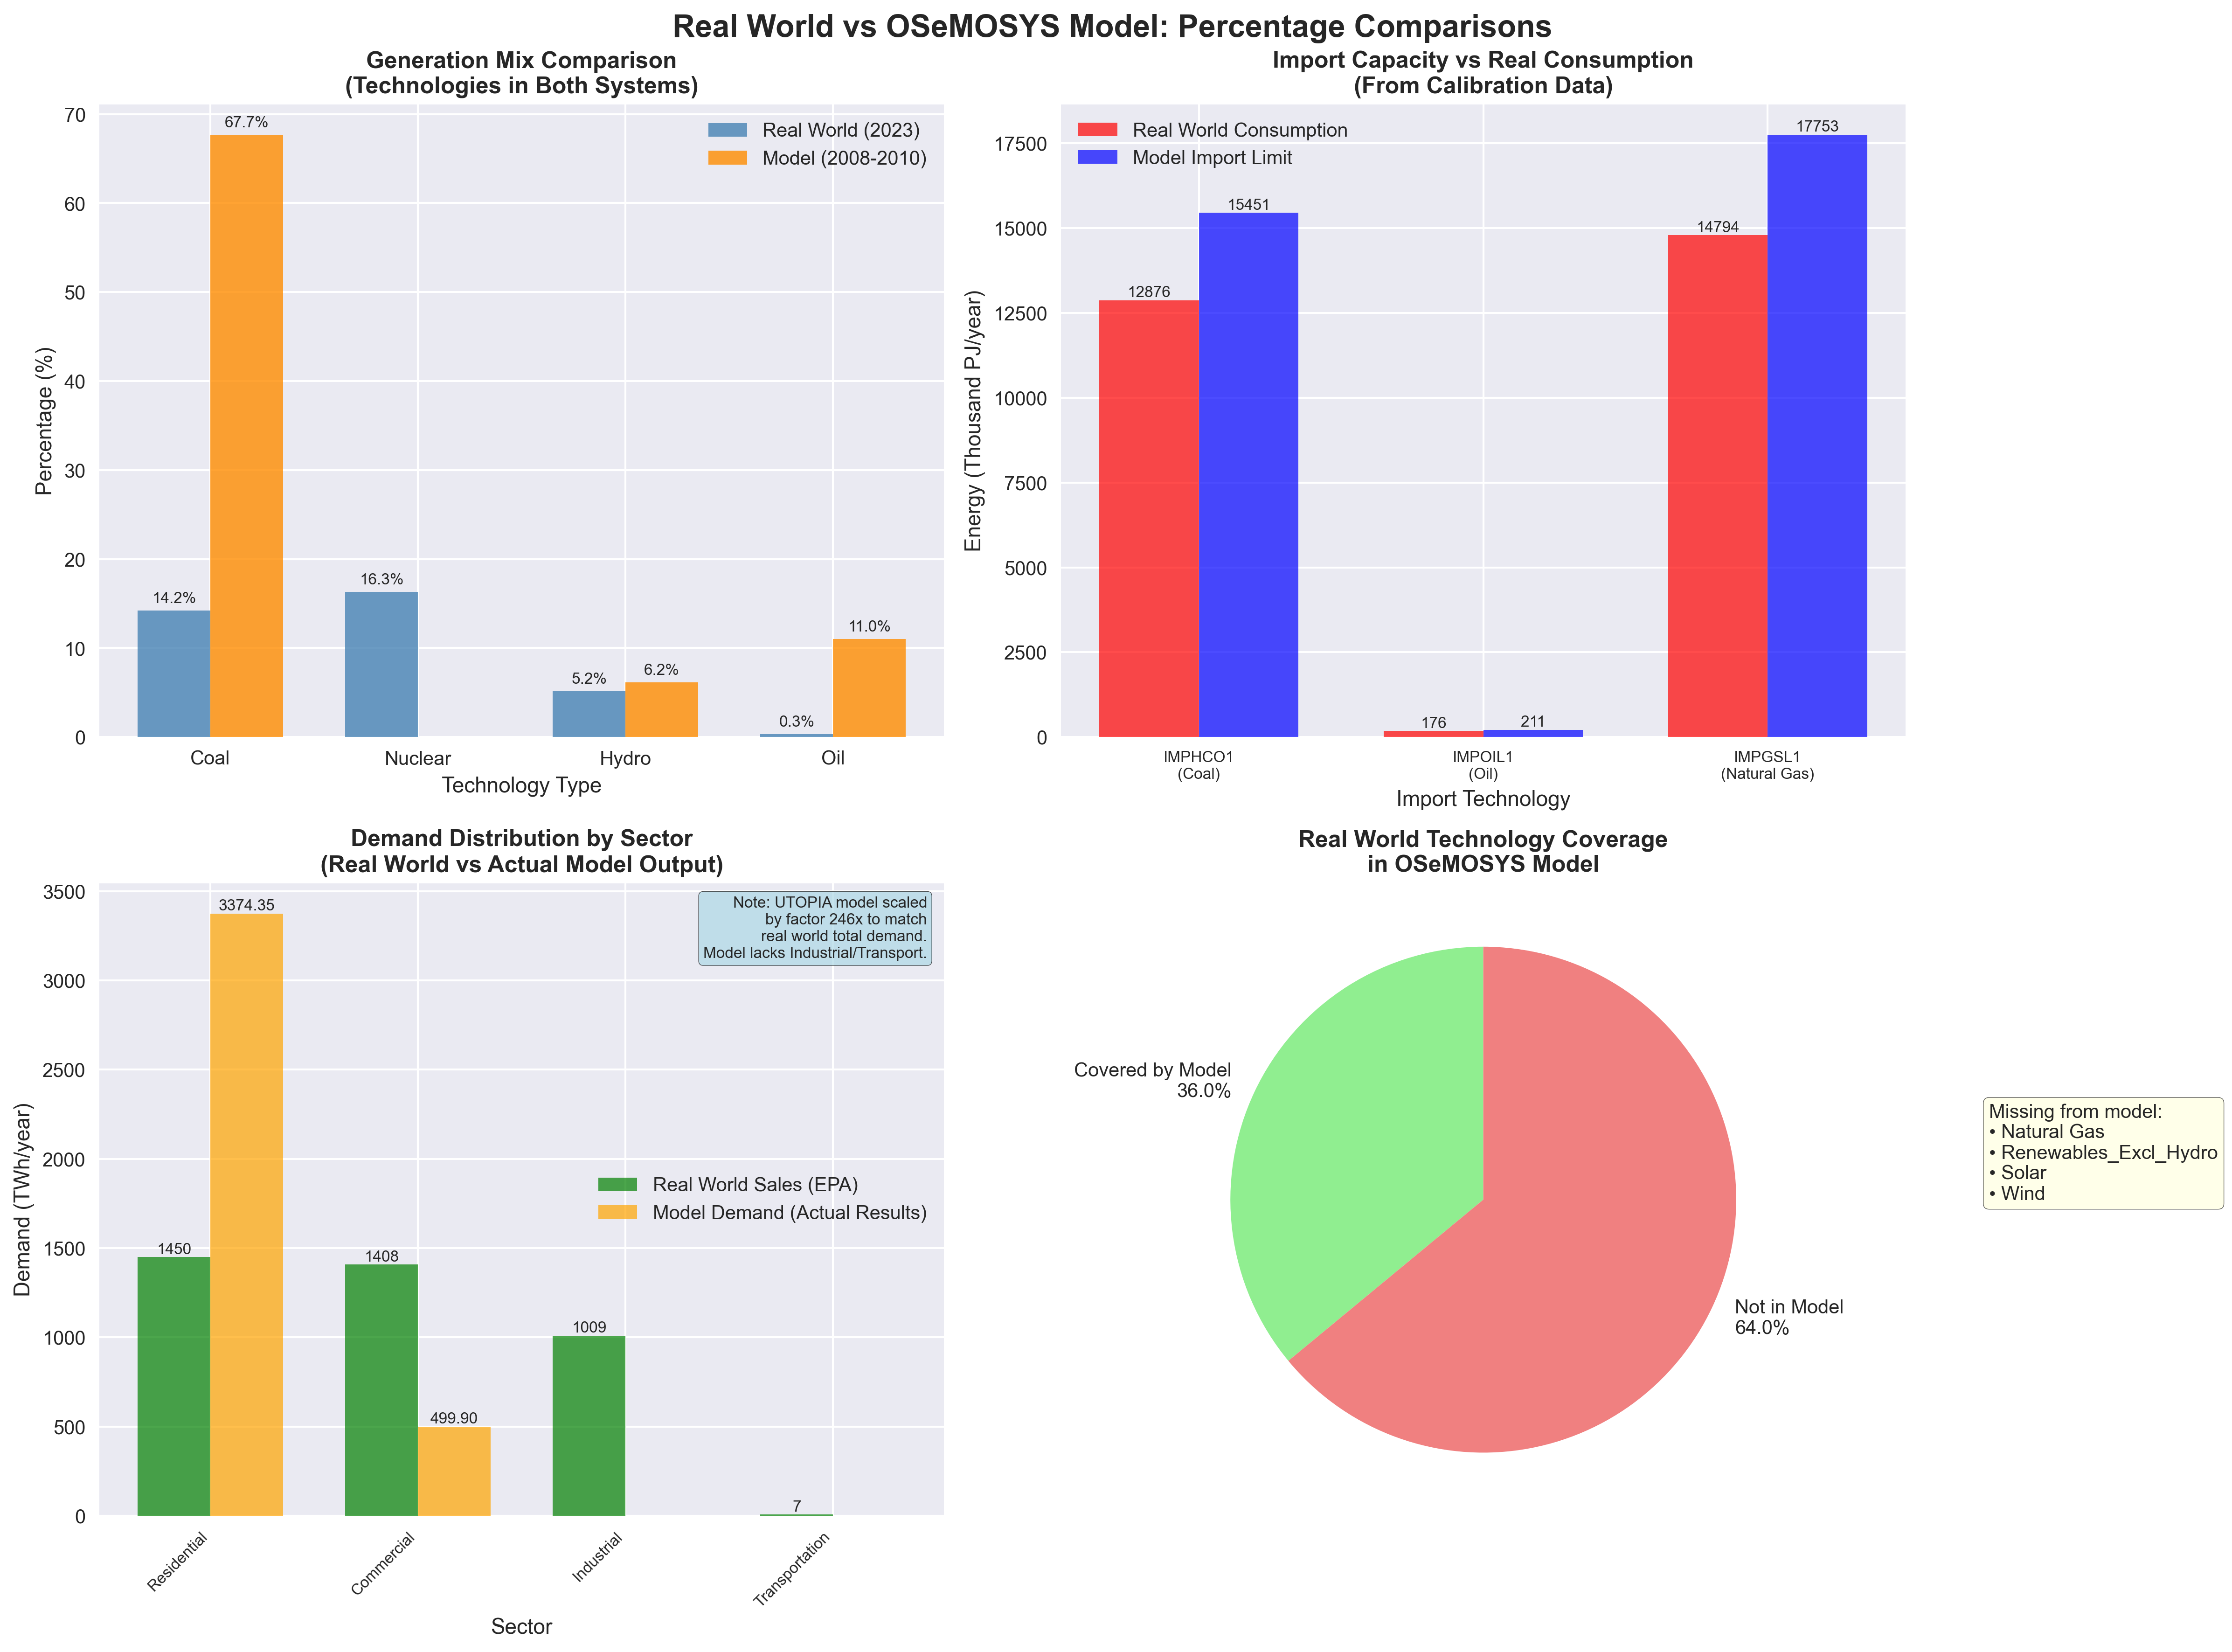
\includegraphics[width=0.8\textwidth]{comparison_output/real_world_vs_model_comparison.png}
    \caption{Comparison of model output with real-world data.}
    \label{fig:real_world_comparison}
\end{figure}

\subsection{Charging and Discharging Efficiencies}
I have added charging and discharging efficiencies parameters, assuming that the charging and discharging processes are 90\% efficient, while the loss rate of storage is 0.005 per time slice. Surprisingly, after adding these parameters, there is no visible change in the model's output as shown in Figure \ref{fig:efficiency_total_cost}, which is the minimized total cost of the energy system. This hints that although in the original functions we define the combined production are no lesser than the combined consumptions, the optimal solution is always to have the two sides equal to minimize the cost. Therefore, adding these efficiencies does not change the optimal solution.

\begin{figure}[H]
    \centering
    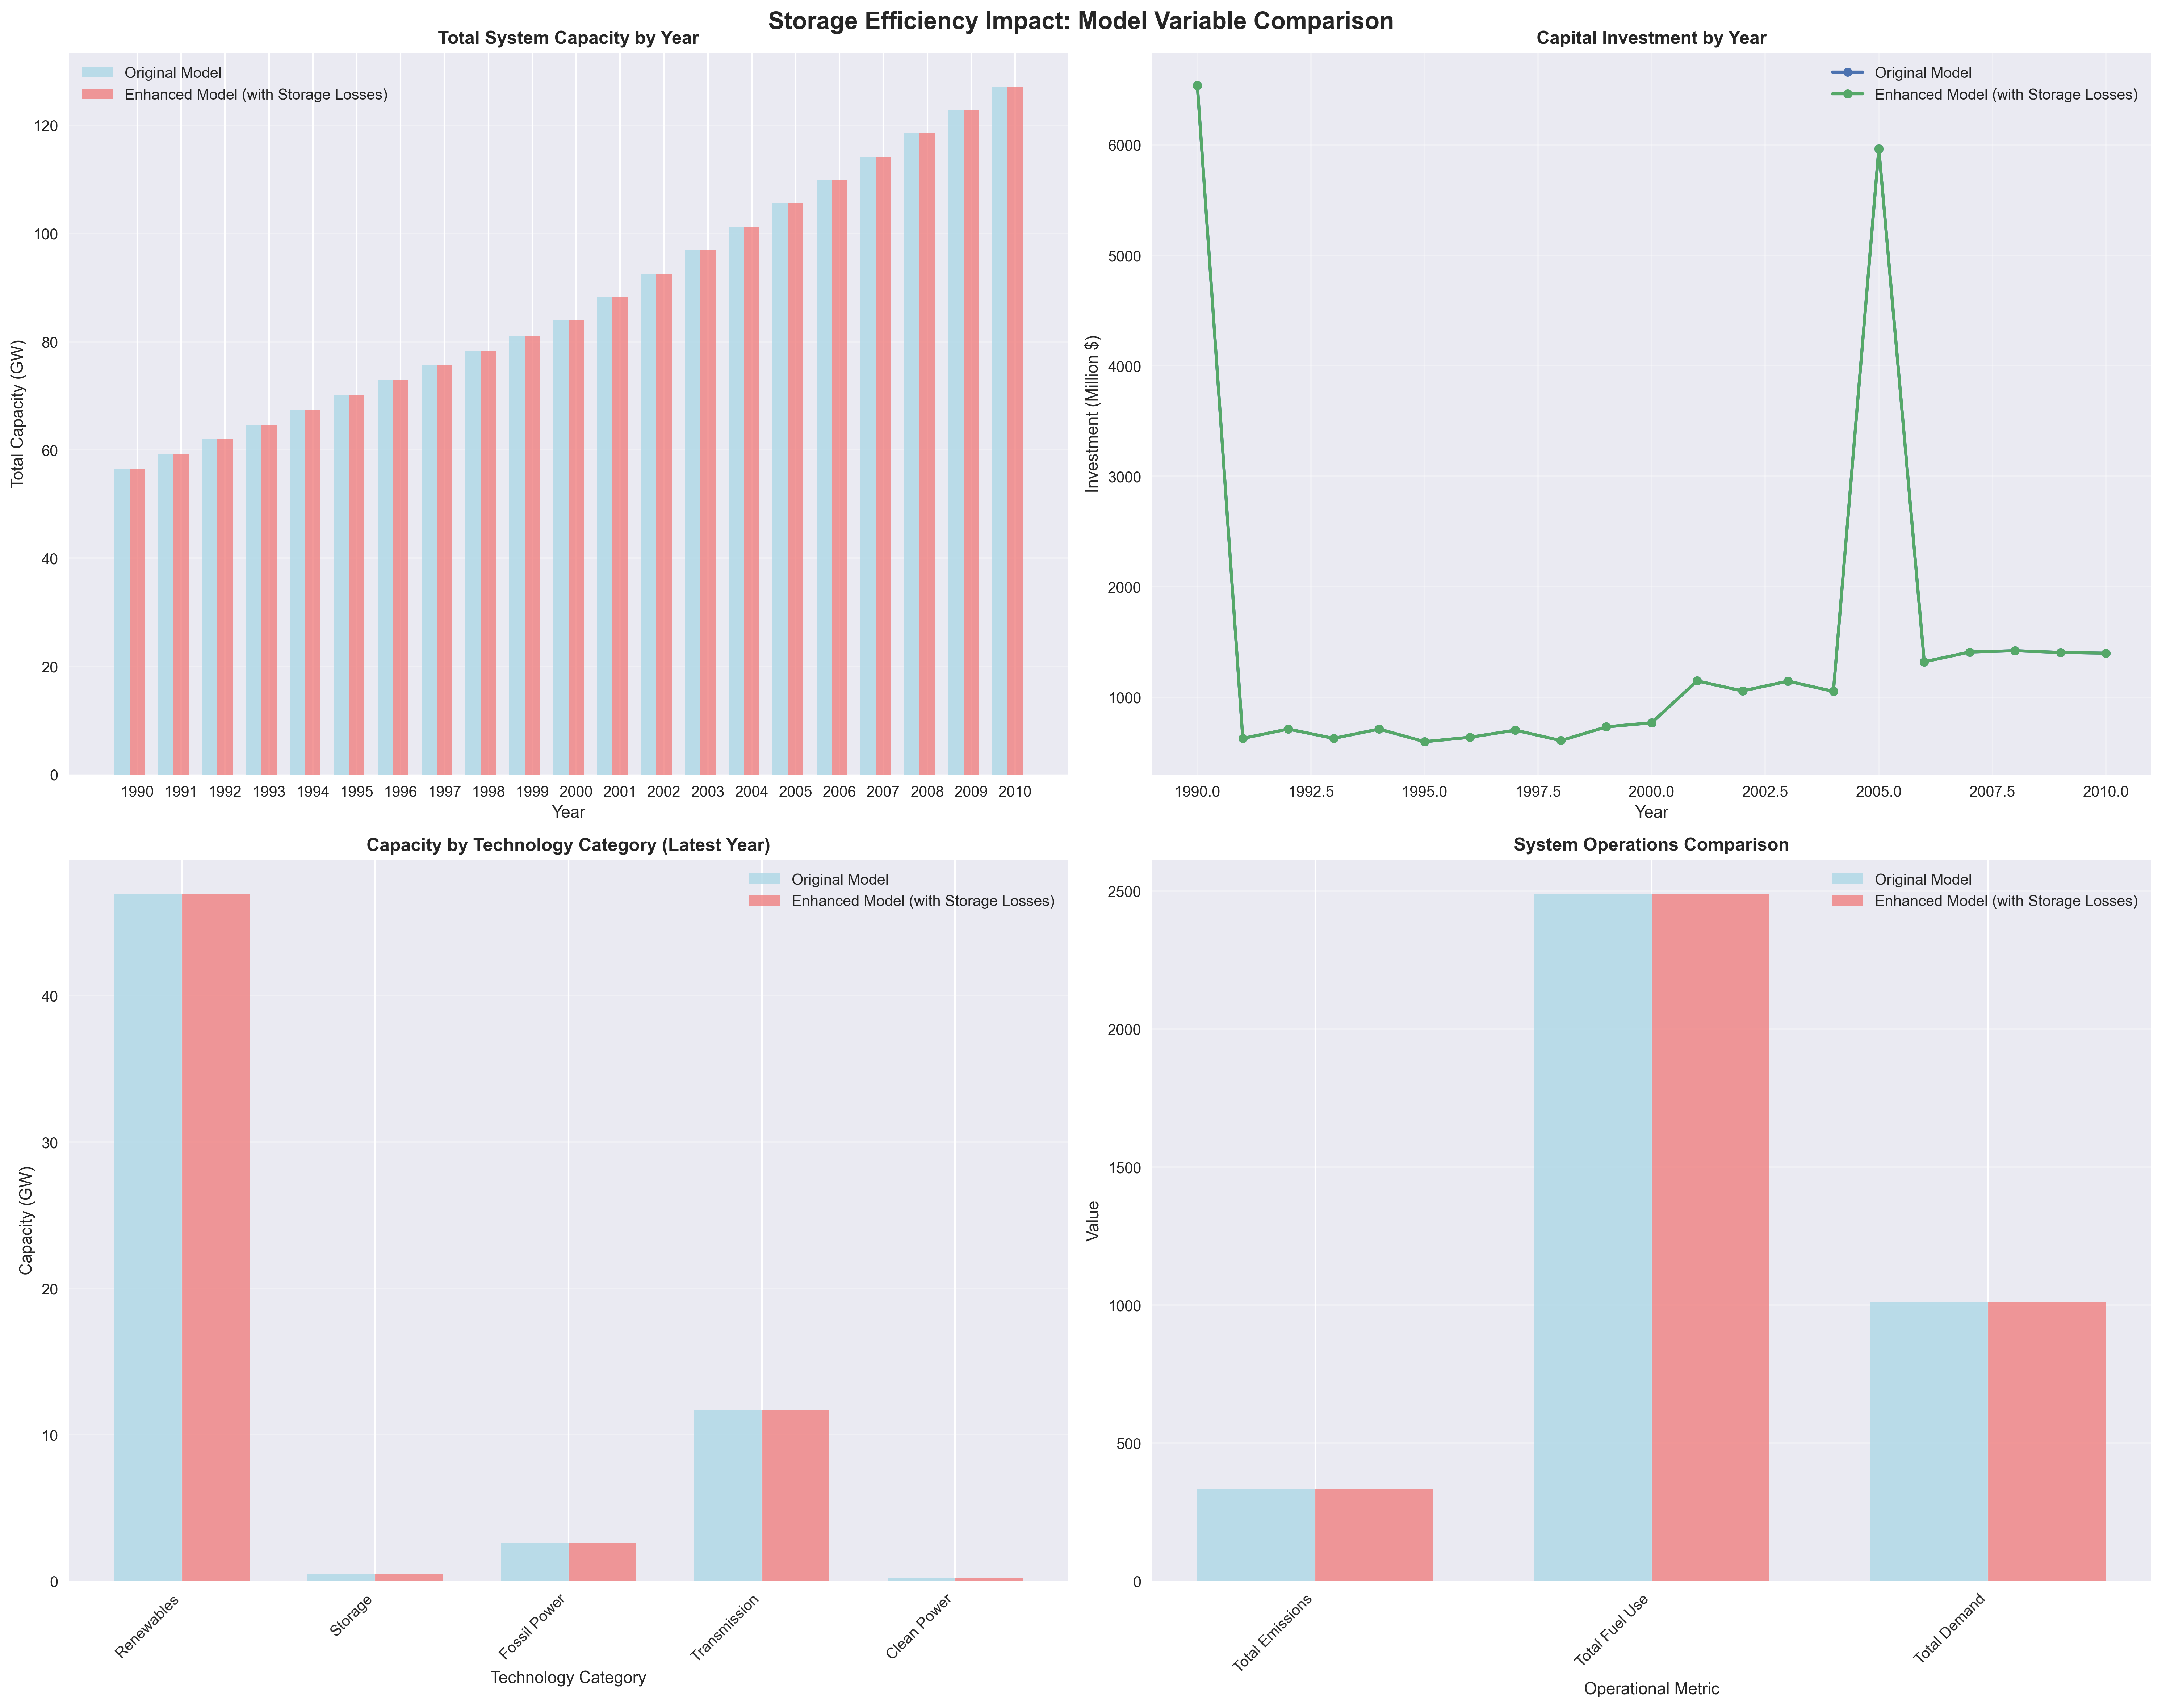
\includegraphics[width=0.8\textwidth]{storage_comparison_output/storage_efficiency_impact_analysis.png}
    \caption{Comparison of total cost with and without charging and discharging efficiencies.}
    \label{fig:efficiency_total_cost}
\end{figure}


\section{Challenges}
Some challenges I face include:
\begin{itemize}
    \item Data Availability: Accessing high-quality, real-world data for model validation is difficult. There are extra efforts needed to convert the data into a format that can be used in the model.
    \item Model Complexity: As I add more features and functionalities, the model may become more complex and harder to solve.
    \item Lack of Verification: There is no real verification as the real-world scenarios do not necessarily follow the minimized cost this model aims to achieve. And there is not guarantee that the model will produce accurate results for all scenarios without proper testing.
\end{itemize}


\bibliographystyle{plain}
\bibliography{references}

\end{document}